\documentclass{beamer}
\usepackage[orientation=portrait,size=custom,width=11.05,height=11.65]{beamerposter}

\usetheme{Boadilla}
\usepackage{comment}
\usepackage{graphicx}
\graphicspath{{../mvp/doc/},{../doc/figs/},{../Nest/doc/},}
\usepackage[absolute,overlay]{textpos}
\setlength{\TPHorizModule}{1cm} % Horizontale Einheit
\setlength{\TPVertModule}{1cm} % Ve
\usepackage{tikz}

\setbeamertemplate{navigation symbols}{}%remove navigation symbols    
\begin{document} 
\begin{frame}[plain,t]{}
	% 	top set of figures
%	\begin{columns}
%		\begin{column}{\textwidth}
%		\centering  
%			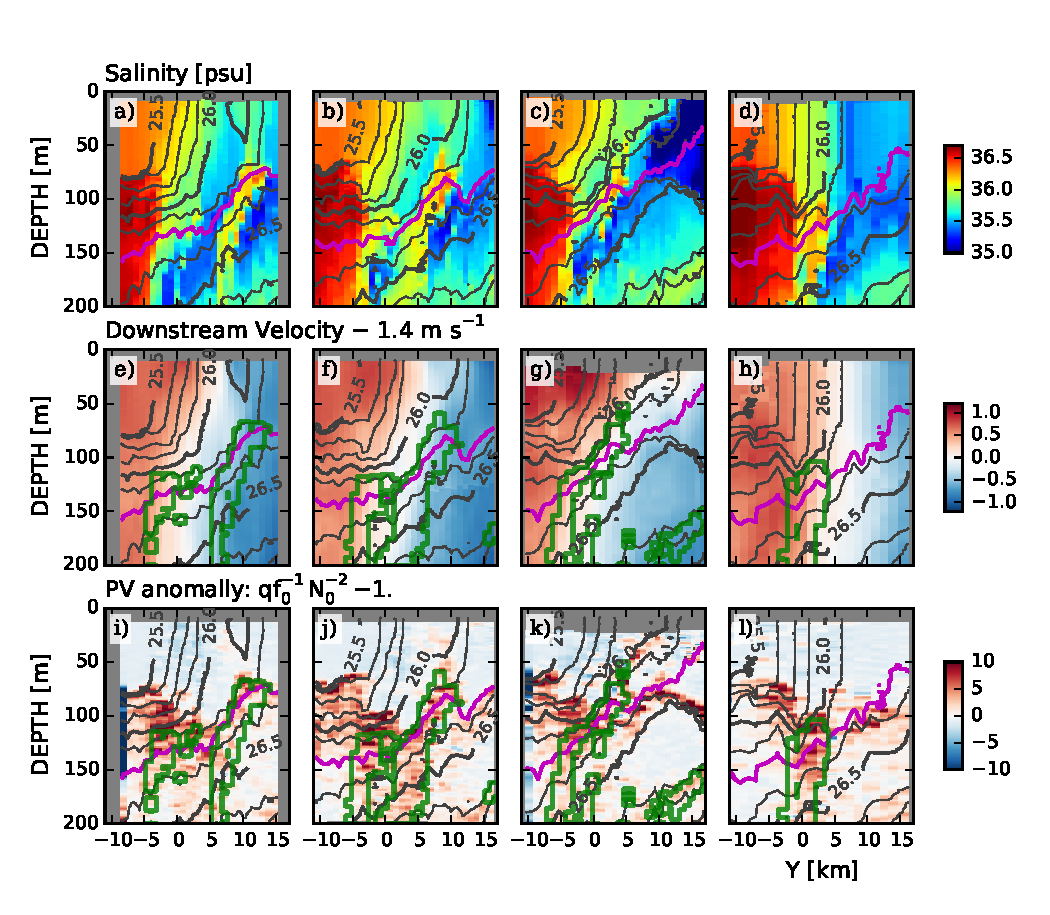
\includegraphics[width=0.95\textwidth,trim=0 10 15 20,clip=true]{SalDFirstStreamer.pdf}
%		
%%			\includegraphics[width=\textwidth]{SalDFirstStreame}
%   
%%			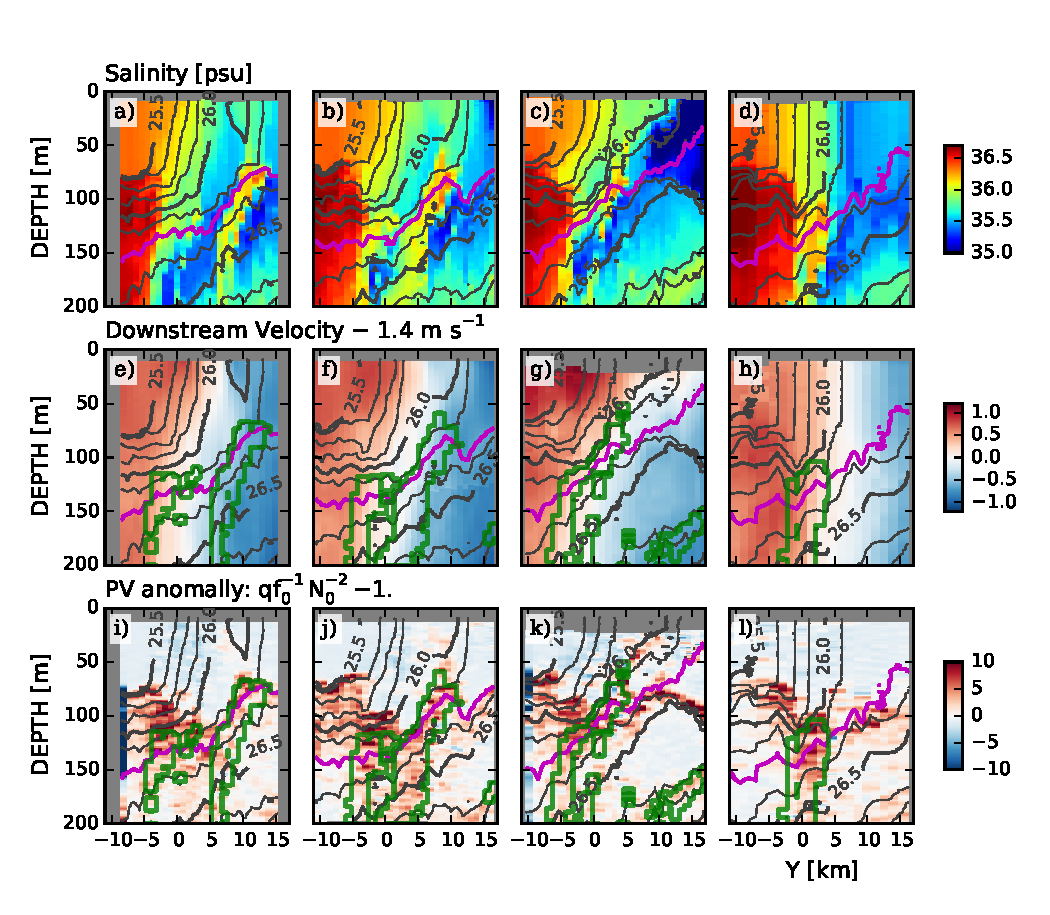
\includegraphics[width=\textwidth]{SalDFirstStreamer}
%		\end{column}
%	\end{columns}
	\centering
	\definecolor{boxcol}{gray}{0.89}
	\begin{textblock}{10}(1.2,1.5)
		%\fcolorbox{black}{boxcol}{
			\begin{minipage}{\textwidth}
			\includegraphics[width=\textwidth]{IsoSurface.pdf}
			\end{minipage}
		%}
	\end{textblock}%
	
	\begin{textblock}{4.9}(0.1,0.)
		\fcolorbox{white}{white}{%
			\begin{minipage}{\textwidth}
			\includegraphics[width=1.065\textwidth,trim=0 0 15 0,clip=True]{TSDensityplot.pdf}
			\end{minipage}
		}
	\end{textblock}%
    \begin{textblock}{10}(0.90,8.5)
		\fcolorbox{white}{white}{%
			\begin{minipage}{\textwidth}
			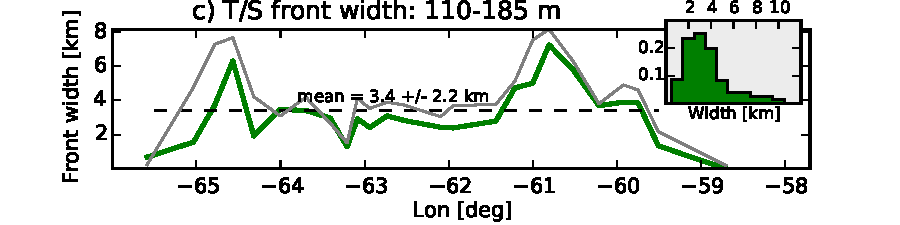
\includegraphics[width=1.052\textwidth,trim=0 0 15 0,clip=True]{FrontWidth.pdf}
			\end{minipage}
		}
	\end{textblock}%
%\centering
%			\includegraphics[width=0.5\textwidth]{TSDensityplot.pdf}\\
%			\includegraphics[width=0.7\textwidth]{IsoSurface.pdf}
	% bottom set of figures.
%\includegraphics[width=\textwidth]{IsoSurface.pdf}
	

\end{frame}
	
\end{document}


